\documentclass[11pt,a4paper]{article}

% --- Codificação e Idioma ---
\usepackage[utf8]{inputenc}
\usepackage[T1]{fontenc}
\usepackage[english]{babel}

% --- Geometria da Página (Margens UAlg: 2.5cm a 3.0cm) ---
\usepackage[top=2.5cm, bottom=2.5cm, left=2.8cm, right=2.5cm]{geometry}
\usepackage{setspace}
\setstretch{1.15}
\setlength{\emergencystretch}{3em}

% --- Matemática e Símbolos ---
\usepackage{amsmath,amssymb}

% --- Tabelas e Gráficos ---
\usepackage{booktabs}
\usepackage{tabularx}
\usepackage{longtable}
\usepackage{graphicx}
\usepackage{float}
\usepackage{caption}
\usepackage{subcaption}
\usepackage{pdflscape}
\usepackage{xcolor}

% --- Formatação de Código ---
\usepackage{listings}
\definecolor{codegreen}{rgb}{0,0.6,0}
\definecolor{codegray}{rgb}{0.5,0.5,0.5}
\definecolor{codepurple}{rgb}{0.58,0,0.82}
\definecolor{backcolour}{rgb}{0.96,0.96,0.96}

\lstdefinestyle{mystyle}{
    backgroundcolor=\color{backcolour},   
    commentstyle=\color{codegreen},
    keywordstyle=\color{magenta},
    numberstyle=\tiny\color{codegray},
    stringstyle=\color{codepurple},
    basicstyle=\ttfamily\footnotesize,
    breakatwhitespace=false,         
    breaklines=true,                 
    captionpos=b,                    
    keepspaces=true,                 
    numbers=left,                    
    numbersep=5pt,                  
    showspaces=false,                
    showstringspaces=false,
    showtabs=false,                  
    tabsize=2,
    frame=single
}
\lstset{style=mystyle}

% --- Cabeçalhos e Rodapés ---
\usepackage{fancyhdr}
\setlength{\headheight}{14pt}
\pagestyle{fancy}
\fancyhf{}
\fancyhead[L]{\small\nouppercase{\leftmark}}
\fancyhead[R]{\small MSc in Informatics Engineering --- UAlg}
\fancyfoot[C]{\thepage}
\renewcommand{\headrulewidth}{0.4pt}
\renewcommand{\footrulewidth}{0pt}

% --- Hiperligações e Metadados ---
\usepackage{xurl}
\usepackage{hyperref}
\hypersetup{
    colorlinks=true,
    linkcolor=blue!70!black,
    citecolor=green!50!black,
    urlcolor=blue!80!black,
    pdftitle={Virtual Data Integration System for Accommodation and Local Discovery in Lisbon - P1},
    pdfauthor={Tiago Vailant, Gonçalo Serafim},
    pdfsubject={Data Modelling and Integration},
    pdfkeywords={Data Integration, Heterogeneity, PostgreSQL, BaseX, XML, MongoDB, Elasticsearch, Airbnb, Tripadvisor}
}

% ==============================================================================
% DOCUMENTO
% ==============================================================================
\begin{document}
\hypersetup{pageanchor=false}

% --- Elementos Pré-Textuais ---
\pagenumbering{roman}
\begin{titlepage}
\begin{center}
\vspace*{-1.0cm}

\includegraphics[width=6.5cm]{ualg_logo.png}\\[0.6cm]
\textsc{\Large University of Algarve}\\[0.2cm]
\textsc{\large Faculty of Sciences and Technology}\\[0.2cm]
\textsc{\small MSc in Informatics Engineering}\\[0.3cm]
\textsc{\small Course Unit: Data Modelling and Integration (14741095)}\\[1.2cm]
\rule{\linewidth}{0.5mm}\\[0.4cm]
{\huge\bfseries Virtual Data Integration System for Accommodation and Local Discovery in Lisbon}\\[0.4cm]
{\Large\bfseries P1 Project Report: Modelling and Populating Heterogeneous Data Sources}\\[0.4cm]
\rule{\linewidth}{0.5mm}\\[1.5cm]
\begin{minipage}{0.48\textwidth}
\begin{flushleft}\large
\emph{Authors:}\\
\textbf{Tiago Alexandre Vailant} (No.\ 79922)\\
\textbf{Gonçalo Serafim} (No.\ 79189)
\end{flushleft}
\end{minipage}\hfill
\begin{minipage}{0.48\textwidth}
\begin{flushright}\large
\emph{Course Coordinator:}\\
\textbf{Professor Paula Cristina Negrão Ventura Martins}
\end{flushright}
\end{minipage}
\vfill
{\large Faro, November 2026}\\[0.2cm]
{\small Academic Year 2026/2027}
\end{center}
\end{titlepage}

\hypersetup{pageanchor=true}
\begin{abstract}
This report presents P1 of a virtual data integration project covering accommodation, restaurants and cultural heritage in Lisbon. Gonçalo Serafim develops guest reviews in Elasticsearch and accommodation listings, owners and price quotes in MongoDB; Tiago Vailant develops restaurants and simulated activity in PostgreSQL and the cultural catalogue in BaseX. The report describes the requirements, conceptual, logical and physical models, provenance, preparation and quality assessment of the four sources. The experiment reproducibly introduces missing values, invalid values and conflicting versions. Owners use synthetic Portuguese Citizen Card or British passport identifiers; activity and document validity are assessed separately. Twelve queries combine both students' subtopics, with explicit conditions, expected results and difficulty criteria. Measured local-source results support preparation of the P2 mediator.

\medskip\noindent\textbf{Keywords:} Virtual data integration, data modelling, heterogeneity, data quality, Lisbon.
\end{abstract}


\newpage
{
\setstretch{1.05}
\tableofcontents
\vspace{0.4cm}
\listoffigures
\vspace{0.3cm}
\listoftables
}
\newpage

% --- Elementos Textuais ---
\pagenumbering{arabic}

\section{Introduction and Context}
\label{sec:introducao}
Planning a stay in Lisbon involves information about accommodation, guest reviews, restaurants and cultural venues. The catalogues have their own structures, identifiers, scales and contacts. Querying them together requires relationships between these elements and explicit treatment of data quality.

The project adopts virtual data integration: each source retains its model, and the P2 mediator will query views over the local systems. P1, the subject of this report, establishes requirements, implements and populates the sources, and defines the contract for future queries, following the assignment\cite{dmi_enunciado2026} and principles of data modelling and integration\cite{lemahieu2018principles,doan2012principles}.

\subsection{Objectives and Method}
The objectives are to represent the two complementary subtopics, justify the technologies, document local models, introduce reproducible quality challenges and specify queries with expected answers. Requirements were formulated from the tourism domain, the available data and the usage scenarios in Section~\ref{sec:requisitos}.

The work distinguishes three outputs: implemented local data and schemas; checks executed against each source; and integrated queries specified for P2. Local measurements and query validation examples have separate sections, respectively Sections~\ref{sec:povoamento_qualidade} and~\ref{sec:consultas}.

\subsection{Responsibilities}
\begin{table}[!htbp]
\centering\footnotesize
\setlength{\tabcolsep}{4pt}\renewcommand{\arraystretch}{1.1}
\caption{Responsibilities, sources and technologies.}\label{tab:divisao_trabalho}
\begin{tabularx}{\textwidth}{>{\raggedright\arraybackslash}p{3.2cm}l>{\raggedright\arraybackslash}p{2.5cm}X}
\toprule
\textbf{Student and subtopic} & \textbf{Source} & \textbf{Technology} & \textbf{Content} \\
\midrule
Gonçalo Serafim (79189), accommodation and guest experience & A1 & Elasticsearch & Textual reviews and account profiles. \\
 & A2 & MongoDB & Listings, host profiles, owners and price quotes. \\
Tiago Vailant (79922), local amenities and activity & B1 & PostgreSQL & Restaurants, labels, group representatives, reservations and visits. \\
 & B2 & BaseX / XML & Museums, monuments and institutional contacts. \\
\bottomrule
\end{tabularx}
\end{table}

\section{Requirements and Use Cases}
\label{sec:requisitos}
\subsection{Glossary and Domain Rules}
\begin{description}
\item[Accommodation listing.] An advertisement with capacity, property type, amenities, location and aggregate ratings in A2.
\item[Review.] A guest comment associated with a listing and an account, with a publication date. This date identifies publication of the comment.
\item[Person.] The source account profile in A1/A2, identified consistently in its author and host roles. In B1, the person is the group representative in the reservation and visit scenario. Each domain retains its own identifier namespace.
\item[Owner.] The host role in A2, modelled as an entity linked to Person. The exercise associates the account responsible for each listing with an owner, a simulated identification document, activity status and a document-validity assessment.
\item[Price quote.] A family of monetary observations from one origin for an accommodation listing. Each observation combines amount, currency, stay dates when known, billing basis, fee inclusion and observation time.
\item[Observation.] Values received for an entity, accompanied by an observation identity, provenance and a timestamp when available. The history preserves versions and repetitions.
\item[Restaurant.] A georeferenced establishment in B1, with cuisine labels and an aggregate rating from the source.
\item[Cultural place.] A B2 record classified as a museum or monument, with location and institutional contacts.
\item[Reservation and visit.] A reservation is an advance restaurant booking. A visit records the group representative's attendance and party size, with an exclusive destination: a restaurant or a cultural place.
\item[Owner activity.] At least one logical review published since 1 January 2025 on any listing belonging to that owner. The scenario assessment uses 13 November 2026 as its reference date.
\item[Proximity.] Approximate geodesic distance between WGS84 coordinates. Listing coordinates include the anonymisation applied by the source; the radius characterises geographical neighbourhood.
\end{description}

\subsection{Actors, Use Cases and Functional Requirements}
Visitors seek accommodation, dining and cultural options. Analysts study the available amenities and recorded activity patterns. Data managers monitor quality and owner identification. Table~\ref{tab:atores_casos_uso} summarises these goals; the precise conditions of each query are specified in Section~\ref{sec:consultas}.

\begin{table}[!htbp]
\centering\footnotesize
\setlength{\tabcolsep}{4pt}\renewcommand{\arraystretch}{1.1}
\caption{Use cases, functional requirements and traceability.}\label{tab:atores_casos_uso}
\begin{tabularx}{\textwidth}{p{2cm}lX p{2cm}}
\toprule
\textbf{Actor} & \textbf{UC / FR} & \textbf{Goal} & \textbf{Validation} \\
\midrule
Visitor & 01 / 01 & Discover restaurants and cultural places near a listing. & Q01--Q04 \\
Visitor & 02 / 02 & Compare affordable listings by nearby dining options. & Q05 \\
Analyst & 03 / 03 & Summarise local amenities by area and monthly restaurant activity. & Q06, Q07 \\
Analyst & 04 / 04 & Relate restaurant and cultural visits to accommodation options. & Q08, Q12 \\
Analyst & 05 / 05 & Study associations between review mentions and local amenities. & Q09 \\
Visitor & 06 / 06 & Select combinations of accommodation, culture and dining with textual evidence. & Q10, Q11 \\
Manager & 07 / 07 & Audit anomalies, histories, references and document validity for active owners. & Section~\ref{sec:povoamento_qualidade} \\
\bottomrule
\end{tabularx}
\end{table}

\subsection{Data Quality Requirements}
The following requirements define the assessment criteria. Section~\ref{sec:povoamento_qualidade} presents the anomalies, applied rules and observed results.
\begin{enumerate}
\item \textbf{DQR-01 --- Validity:} check types, formats and domains for coordinates, ratings, contacts, dates and monetary values.
\item \textbf{DQR-02 --- Completeness:} represent unknown values explicitly and measure their occurrence. Treat latitude and longitude as a pair.
\item \textbf{DQR-03 --- Identity and uniqueness:} maintain one key per logical entity and a unique document identifier per owner. Shared names and contacts require additional evidence for entity matching.
\item \textbf{DQR-04 --- Consistency:} check references, chronology and reservation/visit states, together with agreement between activity, document validity and reference dates.
\item \textbf{DQR-05 --- Semantics:} preserve the scale and context of each rating and price observation.
\item \textbf{DQR-06 --- Provenance:} identify origin, declared licence, acquisition date, generated fields, seeds and the files used in each execution.
\end{enumerate}

\subsection{Non-functional Requirements}
\begin{itemize}
\item \textbf{NFR-01 --- Reproducibility:} prepare, load and verify sources using the requirements and workflow outlined in Appendix~\ref{ap:execucao}.
\item \textbf{NFR-02 --- Autonomy:} retain the four engines and their local schemas; adapters will provide access interfaces for P2.
\item \textbf{NFR-03 --- Robustness:} apply explicit contracts for unknown, invalid and conflicting values, with traceable decisions.
\item \textbf{NFR-04 --- Conventions:} use WGS84 coordinates, ISO 8601 calendar dates and timestamps with explicit time zones. B1 events are presented in Europe/Lisbon; synthetic observation timestamps in A1/A2 are stored in UTC.
\end{itemize}

\section{Sources, Provenance and Technology Choices}
\label{sec:fontes}
\subsection{A1 and A2 --- Accommodation and Reviews}
The supplied Inside Airbnb extracts\cite{insideairbnb} correspond to the Lisbon snapshot of 19 September 2026, acquired on 14 October 2026 under CC BY 4.0. They contain 1\,950\,076 reviews and 25\,020 listings. Originals are preserved and identified by SHA-256 hashes.

A1 organises comment text, publication dates and references to listings and people. A2 organises the accommodation catalogue and price-observation families. Contacts, individual review scores, observation timestamps, owner documents and additional price histories are generated fields for the exercise; aggregate ratings and publication dates retain their extract provenance. Their model and assessment are developed in Sections~\ref{subsec:modelos_goncalo} and~\ref{subsec:qualidade_goncalo}.

Elasticsearch provides inverted indexing, BM25 lexical search, temporal filters and highlighting of matching excerpts. Vector indexing complements this access with similarity search. MongoDB accommodates objects and lists for amenities, location and observations, supporting profile, owner and quote queries through explicit references and local aggregations.

\subsection{B1 --- Restaurants and Activity}
The Lisbon sample of \emph{TripAdvisor European restaurants}, published by Stefano Leone on Kaggle\cite{tripadvisorkaggle}, contains 5\,261 establishments. The extract was selected using \texttt{country = Portugal} and \texttt{city = Lisbon}. It represents a May 2021 snapshot, was acquired on 14 October 2026 and has a declared CC0 licence. Cuisine and venue-type labels produce 12\,167 associations. The activity scenario consists of simulated group representatives, reservations and visits.

PostgreSQL represents relationships between establishments, labels and events, with declarative keys, domains and referential integrity. Cross-table checks complement these constraints. The relational structure and functional dependencies are presented in Section~\ref{subsec:modelos_tiago}.

\subsection{B2 --- Cultural Heritage}
The cultural catalogue contains 130 municipal records for Lisbon: 67 museums and 63 monuments. Data comes from the \emph{Museus} and \emph{Monumentos Nacionais} catalogues, respectively the EquipamentosCulturais ArcGIS service (layer 3) and Patrimonio service (layer 12)\cite{dados_abertos_cml,cml_monumentos}. The recorded access date is 14 October 2026, and both catalogues declare CC0. The cultural catalogue was generated on 15 October 2026 and preserves original identifiers, source attributes and acquisition metadata.

BaseX retains the hierarchical XML structure and supports traversal through XPath and XQuery. The project XSD checks structure, types, domains, place keys and the reference to the origin. Optional contacts and source fields retain the representations specified by the schema.

\clearpage
\section{Conceptual, Logical and Physical Modelling}
\label{sec:modelacao}
\subsection{Tiago Vailant's Source Models (B1 and B2)}
\label{subsec:modelos_tiago}
\paragraph{1. Conceptual Model (ER Diagram):}
The diagram in Figure~\ref{fig:der} structures this subtopic into six entities: \texttt{PESSOA}, \texttt{RESERVA}, \texttt{VISITA}, \texttt{ESTABELECIMENTO}, \texttt{ETIQUETA} (B1) and \texttt{LUGAR\_\allowbreak{}CULTURAL} (B2):
\begin{itemize}\raggedright
\item A \textbf{Person} makes reservations ($0..N$) and participates in visits ($0..N$); only the group representative is identified;
\item Each \textbf{Reservation} belongs to one person ($1$) and one establishment ($1$), and may give rise to at most one completed visit ($0..1$);
\item An \textbf{Establishment} is classified by multiple culinary \textbf{Labels} ($0..N : 0..N$);
\item Each \textbf{Visit} has a mutually exclusive destination: it either takes place at an \texttt{ESTABELECIMENTO} ($0..1$) or at a \texttt{LUGAR\_\allowbreak{}CULTURAL} ($0..1$).
\end{itemize}
Figure~\ref{fig:der} shows the two optional destination relationships separately. Each visit has exactly one destination: an establishment or a cultural place. The exclusive arc is absent from the diagram; the constraint is stated in the text and enforced in PostgreSQL by \texttt{num\_\allowbreak{}nonnulls(\allowbreak{}establishment\_\allowbreak{}id,\allowbreak{} cultural\_\allowbreak{}place\_\allowbreak{}id) = 1}.
\begin{landscape}\begin{figure}[p]\centering
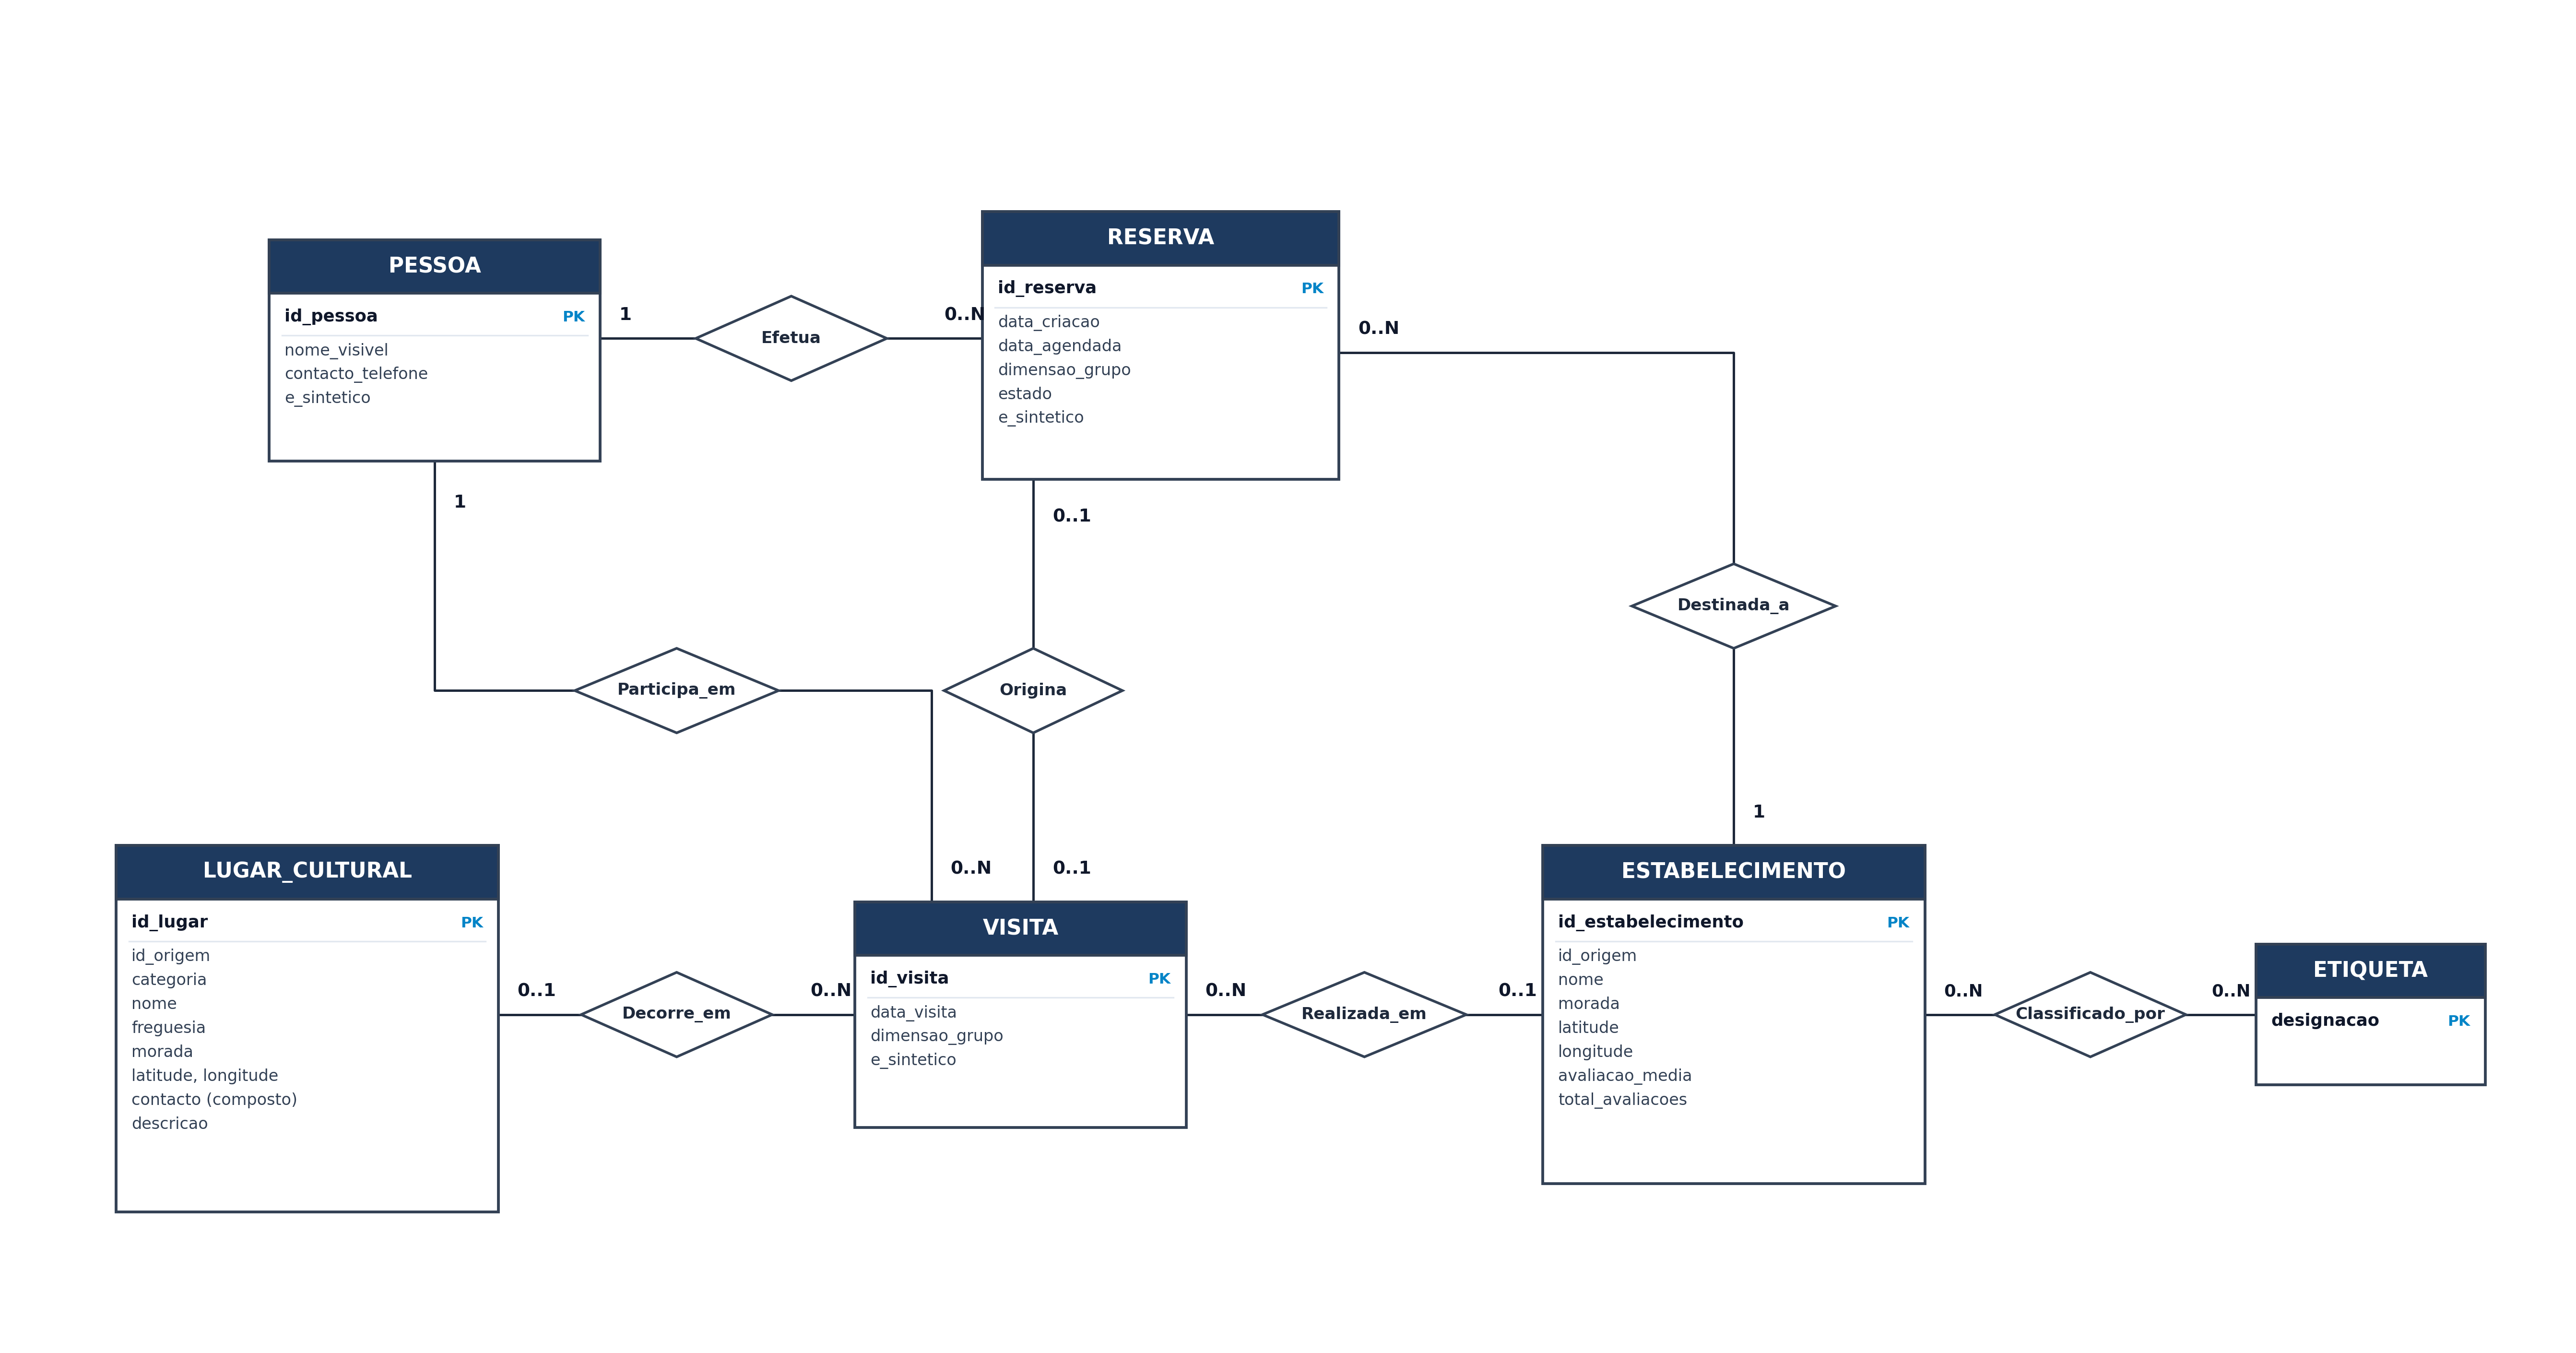
\includegraphics[width=\linewidth,height=0.84\textheight,keepaspectratio]{der_tiago.png}
\caption{Original ER diagram of the local Restaurant, Culture and Activity entities (Tiago Vailant). The English label key follows.}\label{fig:der}
\end{figure}\end{landscape}
\paragraph{English Label Key for Figure~\ref{fig:der}.}
The original diagram retains its Portuguese labels. \texttt{PESSOA} means Person; \texttt{RESERVA}, Reservation; \texttt{VISITA}, Visit; \texttt{ESTABELECIMENTO}, Establishment; \texttt{ETIQUETA}, Label; and \texttt{LUGAR\_CULTURAL}, Cultural Place. Relationship labels translate as follows: \emph{Efetua}, makes; \emph{Destinada\_a}, destined for; \emph{Origina}, gives rise to; \emph{Participa\_em}, participates in; \emph{Decorre\_em}, takes place at; \emph{Realizada\_em}, made at; and \emph{Classificado\_por}, classified by.

Attribute names use \texttt{id} for identifier and \texttt{id\_origem} for source identifier. The remaining labels mean: \texttt{nome\_visivel}, display name; \texttt{contacto\_telefone}, telephone contact; \texttt{e\_sintetico}, synthetic flag; \texttt{data\_criacao}, creation date; \texttt{data\_agendada}, scheduled date; \texttt{dimensao\_grupo}, group size; \texttt{estado}, status; \texttt{data\_visita}, visit date; \texttt{categoria}, category; \texttt{nome}, name; \texttt{freguesia}, parish; \texttt{morada}, address; \texttt{contacto}, contact (\texttt{composto} means composite); \texttt{descricao}, description; \texttt{avaliacao\_media}, average rating; \texttt{total\_avaliacoes}, review count; and \texttt{designacao}, label text. Latitude and longitude retain the same meaning in both languages. The logical schema below gives the corresponding implementation fields.

\paragraph{2. Relational Logical Model and Functional Dependencies (B1):}
The PostgreSQL relational schema \texttt{tiago\_\allowbreak{}lab} comprises five relations, with primary keys underlined and references indicated:
\begin{itemize}\raggedright
\item \texttt{ESTABLISHMENT}(\underline{establishment\_id}, source\_id, name, address, latitude, longitude, average\_rating, review\_count) --- \emph{UK:} \texttt{source\_\allowbreak{}id}
\item \texttt{ESTABLISHMENT\_\allowbreak{}LABEL}(\underline{establishment\_id}, \underline{label}) --- \emph{FK:} \texttt{establishment\_\allowbreak{}id} $\rightarrow$ \texttt{ESTABLISHMENT}
\item \texttt{PERSON}(\underline{person\_id}, display\_name, contact\_phone, is\_synthetic) --- \emph{UK:} \texttt{(\allowbreak{}display\_\allowbreak{}name,\allowbreak{} contact\_\allowbreak{}phone)}
\item \texttt{RESERVATION}(\underline{reservation\_id}, person\_id, establishment\_id, created\_at, scheduled\_at, party\_size, status, is\_synthetic) --- \emph{FKs:} \texttt{person\_\allowbreak{}id} $\rightarrow$ \texttt{PERSON}; \texttt{establishment\_\allowbreak{}id} $\rightarrow$ \texttt{ESTABLISHMENT}; \emph{UKs:} \texttt{(\allowbreak{}person\_\allowbreak{}id,\allowbreak{} establishment\_\allowbreak{}id,\allowbreak{} scheduled\_\allowbreak{}at)}; \texttt{(\allowbreak{}reservation\_\allowbreak{}id,\allowbreak{} person\_\allowbreak{}id,\allowbreak{} establishment\_\allowbreak{}id)}
\item \texttt{VISIT}(\underline{visit\_id}, person\_id, establishment\_id, cultural\_place\_id, reservation\_id, visited\_at, party\_size, is\_synthetic) --- \emph{FKs:} \texttt{person\_\allowbreak{}id} $\rightarrow$ \texttt{PERSON}; \texttt{establishment\_\allowbreak{}id} $\rightarrow$ \texttt{ESTABLISHMENT}; \texttt{(\allowbreak{}reservation\_\allowbreak{}id,\allowbreak{} person\_\allowbreak{}id,\allowbreak{} establishment\_\allowbreak{}id)} $\rightarrow$ \texttt{RESERVATION}; \emph{UKs:} \texttt{reservation\_\allowbreak{}id}; \texttt{(\allowbreak{}person\_\allowbreak{}id,\allowbreak{} visited\_\allowbreak{}at)}
\end{itemize}
\paragraph{3. Identifier and Key Semantics:}
\begin{itemize}\raggedright
\item \textbf{Establishment and Labels:} The natural Tripadvisor key (\texttt{source\_\allowbreak{}id UNIQUE}) is retained for traceability, while joins use the integer \texttt{establishment\_\allowbreak{}id}. The multivalued \texttt{cuisines} column is decomposed into associations keyed by \texttt{(\allowbreak{}establishment\_\allowbreak{}id,\allowbreak{} label)}. In this relation, the attributes form the key; in the remaining relations, descriptive attributes depend on the establishment, group representative or event key. Catalogue normalisation separates label associations from establishment attributes; the visit relation retains the controlled redundancy described below.
\item \textbf{Person (\texttt{PERSON}):} Restaurant bookings and cultural visits do not collect civil identity documents, and neither \texttt{display\_\allowbreak{}name} (namesakes \texttt{"Ana Exemplo"} in IDs \texttt{1} and \texttt{3}) nor \texttt{contact\_\allowbreak{}phone} (shared family number \texttt{"+351910000002"} in IDs \texttt{2} and \texttt{4}) is unique alone. Each group representative is therefore naturally identified by the composite candidate key \texttt{UNIQUE (\allowbreak{}display\_\allowbreak{}name,\allowbreak{} contact\_\allowbreak{}phone)}, while \texttt{person\_\allowbreak{}id} serves as the integer primary key for joins.
\item \textbf{Reservation and Visit:} The keys \texttt{reservation\_\allowbreak{}id} and \texttt{visit\_\allowbreak{}id} identify distinct reservation and visit occurrences, paired with natural composite candidate keys: \texttt{UNIQUE (\allowbreak{}person\_\allowbreak{}id,\allowbreak{} establishment\_\allowbreak{}id,\allowbreak{} scheduled\_\allowbreak{}at)} in \texttt{RESERVATION} (one booking per representative, establishment and scheduled instant) and \texttt{UNIQUE (\allowbreak{}person\_\allowbreak{}id,\allowbreak{} visited\_\allowbreak{}at)} in \texttt{VISIT} (no simultaneous visits by the same representative).
\end{itemize}
Each event key allows repeated reservations or visits by the same group representative to the same place at distinct timestamps. The \texttt{UNIQUE} constraint on the reservation identifier, group representative and establishment provides a superkey supporting the composite foreign key. For visits linked to a reservation, the group representative and establishment repeat the reservation values to allow declarative consistency checks; for walk-in visits, these values identify the event directly. This controlled redundancy and optional reference mean that primary keys alone do not establish 3NF.
\paragraph{4. PostgreSQL Physical Model:}
\begin{itemize}\raggedright
\item \textbf{Domains and Coordinates:} WGS84 bounds, \texttt{average\_\allowbreak{}rating} in $[0, 5]$ (\texttt{numeric(\allowbreak{}2,\allowbreak{}1)}) and mandatory coordinate pairing: \texttt{CHECK (\allowbreak{}(\allowbreak{}latitude IS NULL) = (\allowbreak{}longitude IS NULL))}.
\item \textbf{States and Chronology:} Status is restricted to \texttt{\{'confirmed',\allowbreak{} 'fulfilled',\allowbreak{} 'cancelled',\allowbreak{} 'no\_\allowbreak{}show'\}}, with the invariant \texttt{CHECK (\allowbreak{}created\_\allowbreak{}at <= scheduled\_\allowbreak{}at)}.
\item \textbf{Exclusive Arc and Composite FK:} In \texttt{VISIT}, \texttt{CHECK (\allowbreak{}num\_\allowbreak{}nonnulls(\allowbreak{}establishment\_\allowbreak{}id,\allowbreak{} cultural\_\allowbreak{}place\_\allowbreak{}id) = 1)} ensures a single destination; the composite FK to \texttt{RESERVATION}, together with \texttt{reservation\_\allowbreak{}id UNIQUE}, prevents a completed visit from diverging from its reservation's group representative or restaurant.
\end{itemize}
\paragraph{5. XML Logical and Physical Model in BaseX:}
\begin{itemize}\raggedright
\item \textbf{Hierarchy and Native Key:} The \texttt{<culturalCatalogue>} root groups 130 \texttt{<place>} elements with mandatory attributes \texttt{@id} (pattern \texttt{(\allowbreak{}museum|monument):.+}, uniqueness through \texttt{xs:key} \texttt{placeKey}), \texttt{@category} and \texttt{@sourceRef}, followed by \texttt{<name>}, \texttt{<location>} (\texttt{address}, \texttt{latitude}, \texttt{longitude}, \texttt{parish}), \texttt{<contact>} and \texttt{<description>}.
\item \textbf{Nullability and Cross-DBMS Link:} Contact and description subelements declare \texttt{nillable="true"} (\texttt{xsi:nil="true"}), distinguishing explicit absence from omission of \texttt{<fax>}. Column \texttt{visit.cultural\_\allowbreak{}place\_\allowbreak{}id} (B1) references \texttt{place/@id} (B2) across autonomous engines.
\end{itemize}
The XML schema also includes \texttt{sources/source} metadata, keyed by \texttt{sourceKey}, and the \texttt{placeSource} reference from \texttt{place/@sourceRef} to that key. The \texttt{sourceFields} block preserves raw source attributes. Quality checks also verify agreement between category, identifier prefix and source reference.

Reservation--visit rules are verified by audit queries: \texttt{fulfilled} status, a visit after reservation creation, matching group size and a visit for each fulfilled reservation. Cultural reference checks compare B1 against XML identifiers. Distinguishing declarative constraints from audits locates responsibility for each check.
The XSD is applied by the catalogue preparation and verification process. The BaseX database permits subsequent changes, which require those checks to be rerun; the schema is not automatically reapplied to every write. Raw \texttt{sourceFields} values are retained without specific validation. Agreement between category, source and identifier prefix is audited using XQuery. For contacts, checks measure structure and completeness; telephone normalisation in integrated queries follows the contract planned for P2.
\subsection{Gonçalo Serafim's Source Models (A1 and A2)}\label{subsec:modelos_goncalo}
\subsubsection{Conceptual Model and Identity}
The model in Figure~\ref{fig:der_goncalo} comprises Person, Owner, Accommodation, Review and Price Quote. Each owner corresponds to one person; a person may assume the owner role. An owner has one or more accommodations, and each accommodation has one owner. Each review has one author and one accommodation. An accommodation receives zero or more reviews and has zero or more quote families.

Person identifies the source account profile. The same account retains its key in the author and host roles. The link to Owner brings together document identification and activity indicators. Relationships use keys: \texttt{person\_\allowbreak{}id} derives from the original account; \texttt{owner\_\allowbreak{}id} identifies its owner role; \texttt{listing\_\allowbreak{}id} identifies the listing. The review key combines the listing and original comment identifier, in the form \texttt{R<listing>-<comment>}. Histories belong to the observed entity as multivalued composite attributes.

The document forms an alternate Owner key: issuing country, type and number, represented by \texttt{document\_\allowbreak{}key}. The technical key preserves references when document details are updated. The exercise maintains consistent document identification for each owner in each preparation run.

In the figure, indentation shows the components of a composite attribute; 1..N indicates a multivalued collection. In Price Quote, the monetary context, timestamp, received values and quality indicators belong to each observation. In Owner, the alternate key uses document country, type and number; nationality is a component of the document profile. Derived states use the reference dates specified in the logical model.
\begin{landscape}\begin{figure}[p]\centering
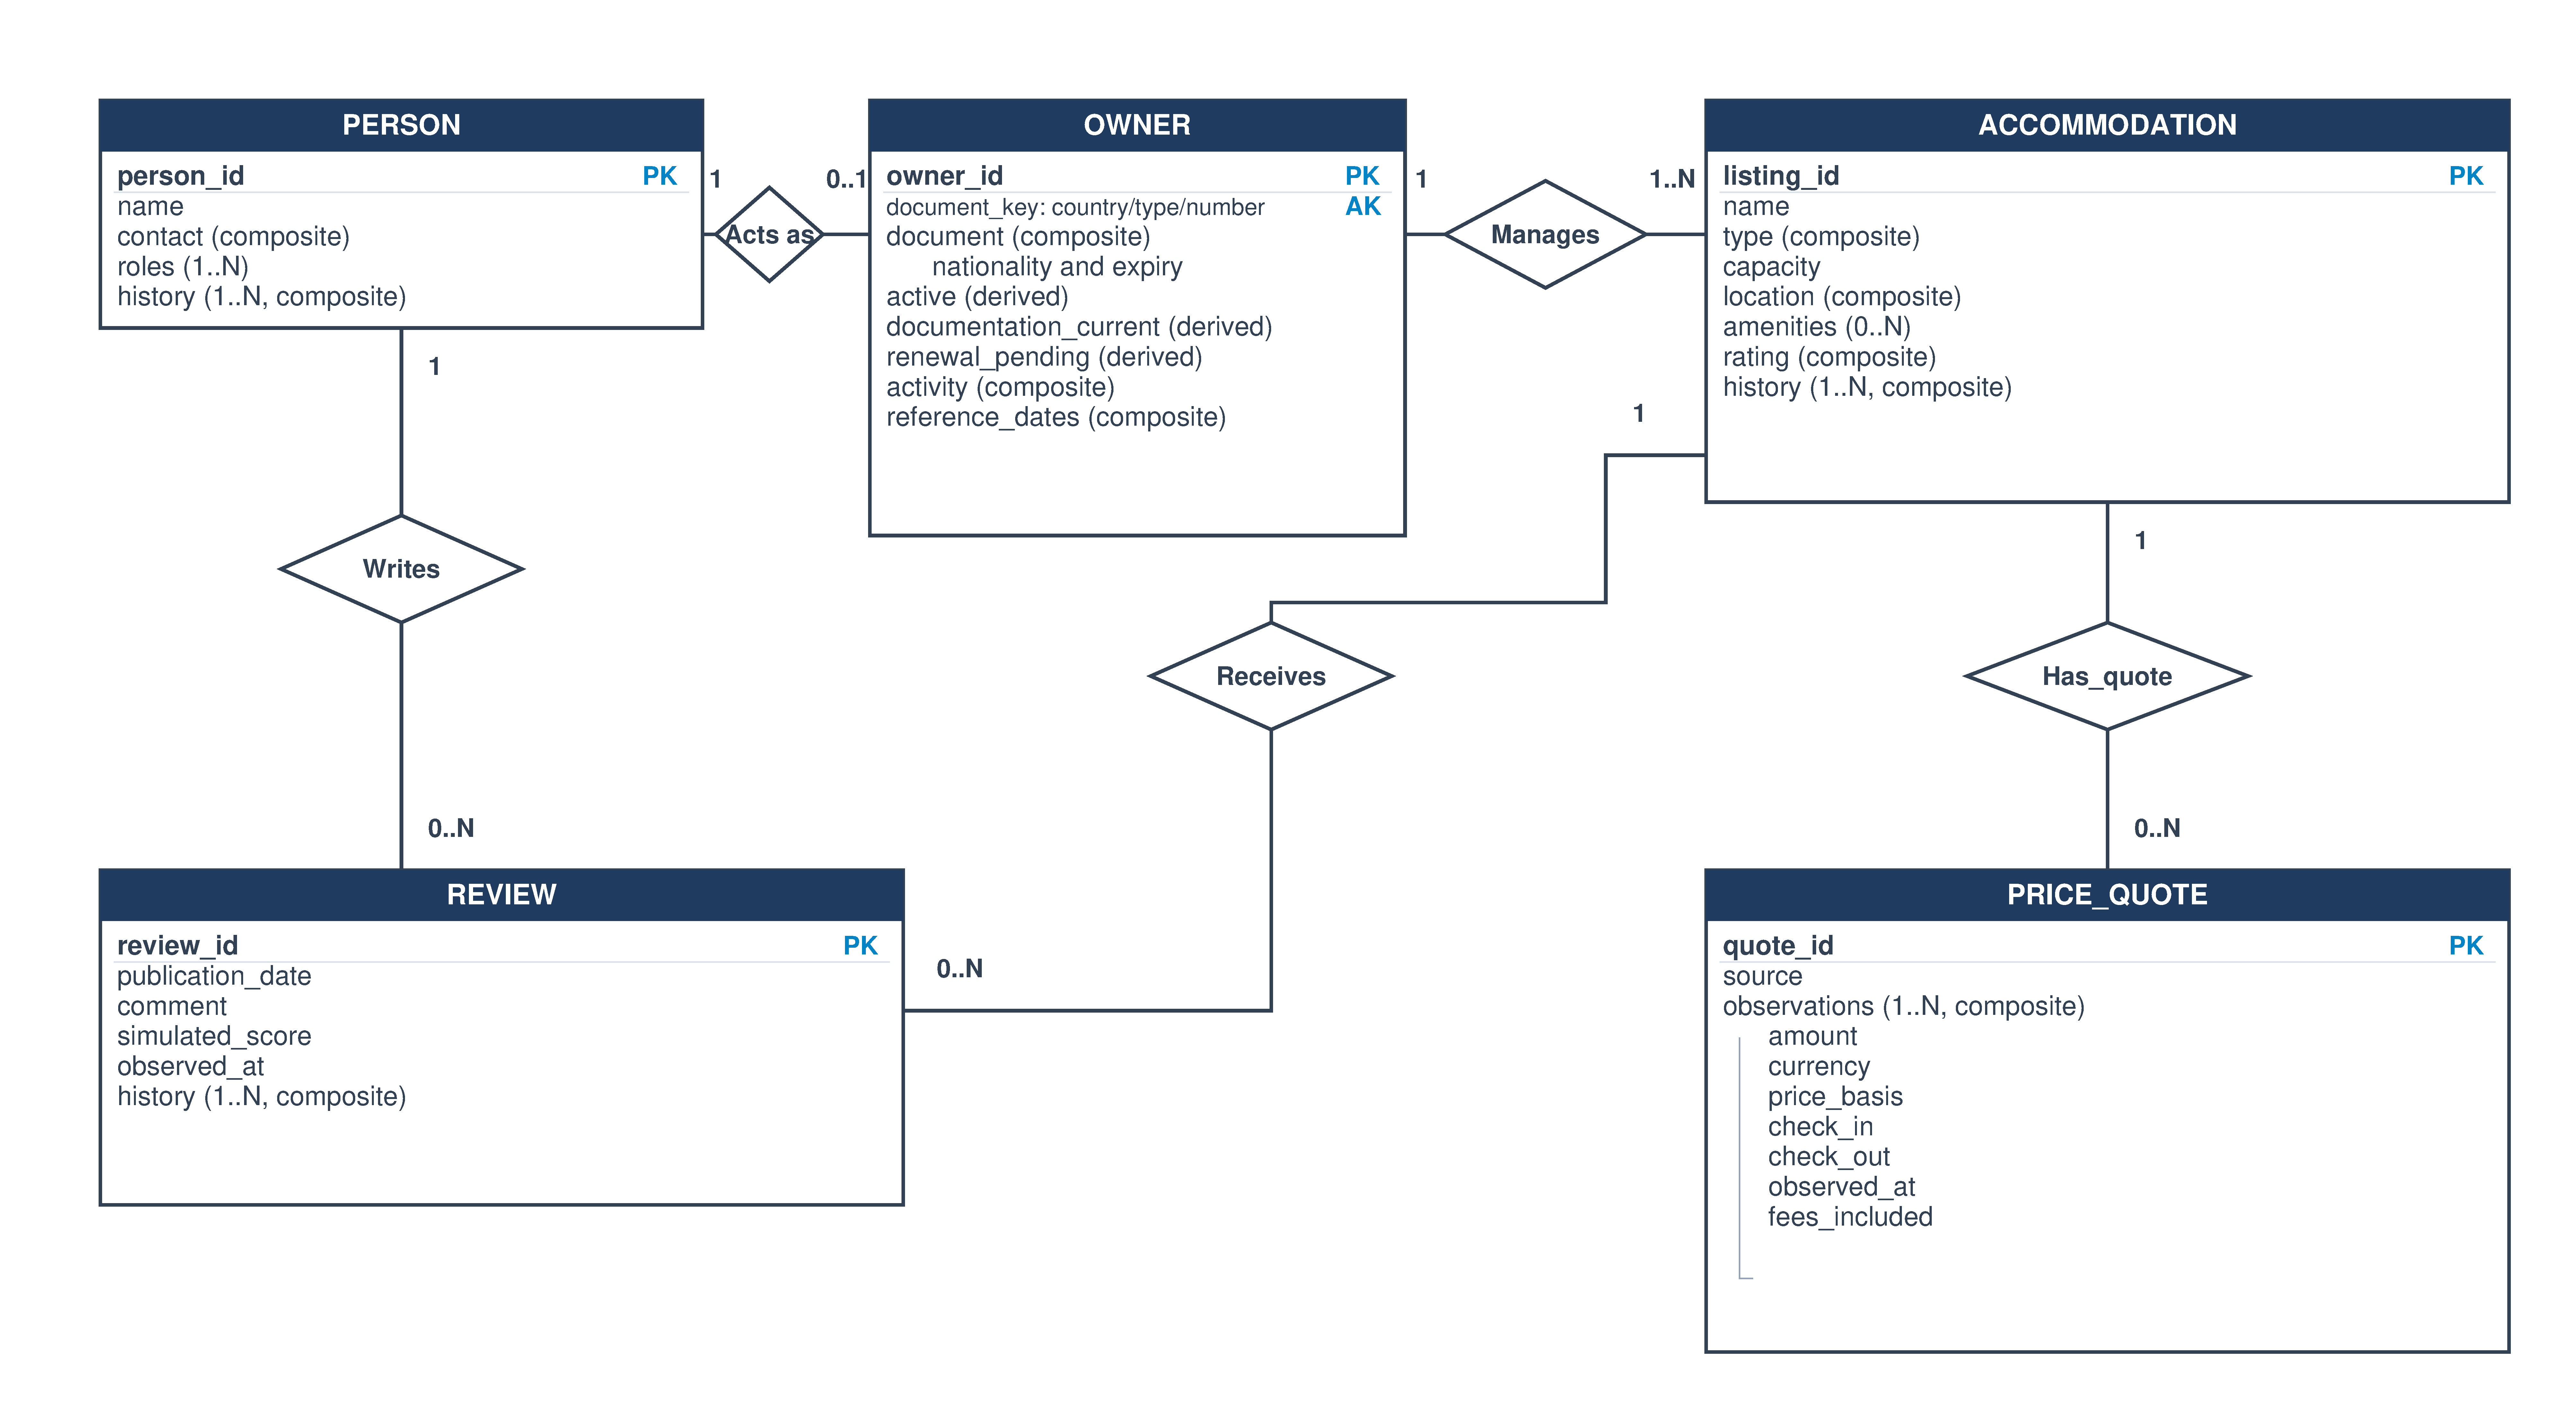
\includegraphics[width=\linewidth,height=0.84\textheight,keepaspectratio]{der_goncalo_owner_en.pdf}
\caption{ER diagram of the local Accommodation, Review, Owner and Price Quote entities (Gonçalo Serafim).}\label{fig:der_goncalo}
\end{figure}\end{landscape}
\subsubsection{Owner, Document and Derived States}
Owner references Person and brings together \texttt{identity\_\allowbreak{}document}, activity and the indicators \texttt{active}, \texttt{documentation\_\allowbreak{}up\_\allowbreak{}to\_\allowbreak{}date} and \texttt{needs\_\allowbreak{}renewal}. The activity block stores the number of accommodations, recent review count, latest known publication date, period start and assessment date.

Activity is calculated from logical reviews since 1 January 2025, summed across the owner's accommodations. A positive count determines \texttt{active = true}. Document validity compares the reference date with \texttt{expires\_\allowbreak{}on}: the document remains valid throughout its expiry date and requires renewal from the following day. Thus, an active owner may have an outstanding document renewal, and an inactive owner may hold up-to-date documentation.

The scenario generates Portuguese and British nationalities independently of the telephone contact's country. Synthetic Portuguese Citizen Card identifiers follow the official structure and check-digit rules\cite{cc_formato}, while British passport identifiers contain nine digits\cite{passport_formato}. Identifiers are stored as text, remain unique across owners and are explicitly distinguished from real personal data.

Document dates use the calendar domain 1900--2199, suitable for representing future expiry dates in the scenario. Document identifiers are critical information: preparation produces valid, unique numbers, and pre-validation rejects missing or invalid documents, documents shared by different accounts, and inconsistent documents for the same owner.

Persisted document indicators form a snapshot dated by \texttt{status\_\allowbreak{}as\_\allowbreak{}of}. Queries recalculate validity for the requested date, defaulting to the current date. Activity retains the assessment date of the prepared dataset. The two dates allow the currency of the indicators to be interpreted separately.
\subsubsection{A1 Logical and Physical Model}
The review index contains one record per logical review, bringing together its accommodation, author, publication date, comment, simulated score, history and quality indicators. A separate person index stores account profiles and contact information. Owner identification is maintained in A2 and represented consistently in A1.

Lexical search uses BM25 to rank matching comments and highlight relevant excerpts. Optional semantic search uses Qwen3-Embedding-4B to represent comments as 1\,024-dimensional vectors, compared using cosine similarity. Raw histories remain available for inspection, while searches operate on canonical values.
\subsubsection{A2 Logical and Physical Model}
The accommodation database organises information into four collections: accommodations, people, owners and price quotes.
\begin{description}
\item[\texttt{accommodation}.] Key \texttt{listing\_\allowbreak{}id}; references \texttt{owner\_\allowbreak{}id} and \texttt{host\_\allowbreak{}person\_\allowbreak{}id}; name, type, capacity, amenities, location, ratings, review summary and history. GeoJSON positions use longitude--latitude order.
\item[\texttt{people}.] Host account profiles, identified by \texttt{person\_\allowbreak{}id}, with name, contact country and national number, roles and observations. A1's contact representation includes the country calling code; A2 stores country and national number separately.
\item[\texttt{owners}.] Technical keys \texttt{owner\_\allowbreak{}id} and \texttt{person\_\allowbreak{}id}, document identification, activity, validity and assessment dates. Uniqueness is enforced on each of these references and on the document key.
\item[\texttt{price\_\allowbreak{}quotes}.] Key \texttt{quote\_\allowbreak{}id}, reference \texttt{listing\_\allowbreak{}id}, source and observation list. Each observation preserves its original, normalised values and quality indicators. Normalised amounts use Decimal128.
\end{description}
Strict validators check types and permitted fields. Canonical coordinates are both known or both null; valid locations have a \texttt{2dsphere} index. Canonical dates are BSON dates. Unique indexes protect keys, while load validation checks cross-document references and consistency of the owner projection in A1. Owner validation expressions check CC check digits, consistency between country, type and number, and agreement of derived states with stored counts and dates.
\subsubsection{Quotes and Query-Time Resolution}
The monetary context is the tuple \( (\text{amount},\text{currency},\text{check-in},\text{check-out},\text{basis},\text{fees}) \). A usable monetary observation has a finite, non-negative amount, currency in EUR/GBP/USD, and basis \texttt{unspecified}, \texttt{per\_\allowbreak{}night} or \texttt{per\_\allowbreak{}stay}. Dates and fee inclusion may remain unknown. Selection preserves the entire tuple of the chosen observation.

Under \texttt{agreement-only}, a quote is resolved when all usable tuples agree. Policy \texttt{latest-valid} accepts the same agreement case; where values differ, it requires known timestamps for every usable observation and agreement among observations at the latest timestamp. A conflicting tie or a conflict with incomplete chronology yields an \emph{unresolved} state. Absence of usable observations yields an \emph{unavailable} state.

The prepared source data retain reference amounts with basis \texttt{unspecified} and unknown fee inclusion. Queries with price limits compare this resolved amount in EUR. The catalogue's mean price represents the mean of these reference amounts. The additional \texttt{simulated} scenario declares nightly amounts and stay dates. Date-based searches compare requested dates with the context selected by the policy. Observations, including exact copies, remain available throughout the process.

\section{Preparation and Quality Assessment}\label{sec:povoamento_qualidade}
The experiment combines external data with generated scenarios that exercise quality rules. Preparation preserves originals and produces working inputs with controlled changes. Loading validates and reconciles observations, retaining received values and the reasons for decisions. This separation allows comparison of source information, introduced anomalies and queryable values.
\subsection{Population and Evidence}
In B1, catalogue selection and label decomposition precede loading of the reservation and visit scenario. In B2, the XML copy is validated against the XSD and loaded into BaseX. Tiago's tests were run up until November 16th: 16 catalogue checks, 38 catalogue-with-activity checks and 36 XML/BaseX checks. For A1/A2, full tests on 13 November verify preparation, references, validators, local queries and the owner model.
\begin{table}[!htbp]\centering\footnotesize\setlength{\tabcolsep}{4pt}\renewcommand{\arraystretch}{1.1}
\caption{Size of the prepared sources and histories.}\label{tab:contagens}
\begin{tabularx}{\textwidth}{lXr}\toprule\textbf{Source} & \textbf{Object or observation} & \textbf{Count} \\\midrule
A1 & Logical reviews / review observations & 1\,950\,076 / 1\,964\,992 \\
A1 & Person profiles & 1\,762\,796 \\
A2 & Accommodations / accommodation observations & 25\,020 / 25\,208 \\
A2 & Host profiles / owners & 9\,484 / 9\,484 \\
A2 & Quote families / monetary observations & 23\,661 / 24\,861 \\
B1 & Restaurants / label associations & 5\,261 / 12\,167 \\
B1 & Simulated group representatives / reservations / visits & 12 / 19 / 28 \\
B2 & Museums / monuments & 67 / 63 \\\bottomrule\end{tabularx}\end{table}
\subsection{B1/B2 Activity and Quality Scenario}
The synthetic activity scenario contains 12 group representatives, 19 reservations and 28 visits in September and October 2026, assessed against a reference date of 21 October:
\begin{itemize}
\item \textbf{Reservations (19):} 12 \texttt{fulfilled} (each linked to one completed visit), 3 future \texttt{confirmed} reservations without a visit, 2 \texttt{cancelled} and 2 \texttt{no\_\allowbreak{}show} (with no \texttt{visit} entry);
\item \textbf{Visits (28):} 12 linked to fulfilled reservations, nine walk-in restaurant visits and seven cultural visits, comprising three visits to one monument and four to one museum.
\end{itemize}
\subsubsection{Tiago Vailant's Sources (B1 and B2)}
\begin{enumerate}
\item \textbf{Incompleteness and Spatial Outliers in B1:} The data preserve 89 restaurants without coordinates (paired \texttt{NULL}s), 450 without an average rating, 6 without a review count and 811 without labels. Some records have coordinates outside Lisbon, including locations in northern Portugal and Almada; distance-based filtering excludes these from local results.
\item \textbf{Composite Contacts, Syntax Errors and Nulls in B2:} Across 130 cultural places there are 57 \texttt{xsi:nil="true"} telephone numbers, 59 null emails, 59 null websites, 3 null descriptions and, for \texttt{fax}, 67 \texttt{xsi:nil="true"} values alongside 63 omitted nodes. The 73 populated telephone fields include extensions and multiple numbers (e.g. \texttt{"+351 213 250 800 / 835"}, \texttt{"21 301 12 82/ 21 301 16 75/21 301 11 28"}) and irregular spacing (\texttt{"+ 351 217 823 474"}), alongside an email with a double \texttt{@} (\nolinkurl{info@info@casa-museumedeirosealmeida.pt}).
\item \textbf{Namesakes and Multi-Category Records (B1 and B2):} B1 contains 95 groups of distinct restaurants sharing a name (e.g. 24 \emph{A Padaria Portuguesa}, 8 \emph{Starbucks}, 2 \emph{Tasca do Manel}) and group representatives with the same name (\texttt{"Ana Exemplo"}, IDs \texttt{1} and \texttt{3}) or shared family contact numbers (\texttt{"+351910000002"}, IDs \texttt{2} and \texttt{4}), which are uniquely disambiguated by the composite natural key \texttt{(display\_name, contact\_phone)}. B2 contains 4 repeated-name pairs: two within \texttt{museum} (\emph{Museu Nacional dos Coches}, \emph{Museu de Lisboa -- Palácio Pimenta}) and two registered as both \texttt{monument} and \texttt{museum} (\emph{Palácio Fronteira} and \emph{Palácio Nacional da Ajuda}).
\item \textbf{Toponymic Granularity (B1 vs B2):} B2 uses the administrative division into 24 parishes represented in the catalogue (\texttt{"Santa Maria Maior"}, \texttt{"Misericórdia"}), while B1 uses free-text addresses and historic neighbourhoods (\texttt{"Chiado"}, \texttt{"Bairro Alto"}), requiring spatial joins using WGS84 coordinates.
\end{enumerate}
\subsection{Injection and Treatment in A1/A2}\label{subsec:qualidade_goncalo}
Fixed random seeds make the generation of contacts, quality anomalies, individual scores and price scenarios reproducible. Approximately 5\% of review and accommodation families are selected. Each selected family receives one, two or three groups of changes with probabilities of 80\%, 17\% and 3\%. Selection covers 97\,359 reviews (4.99\%) and 1\,328 accommodations (5.31\%). These figures measure generator intervention; existing incompleteness is profiled separately.
\begin{description}
\item[Missing Values and Domains.] Small fractions of texts, names, telephone numbers, prices, ratings, amenities and dates are removed. Spatial anomalies include missing coordinate pairs and out-of-range coordinates. Introduced anomalies include short telephone numbers, calling code \texttt{+999}, unknown contact country, latitude 999, negative price and rating 9 on a 0--5 scale. The incompatible canonical field becomes null, while history retains the received value. An unusable critical identity places the record in quarantine; owner documentation is checked before source replacement.
\item[Representation.] Contacts with \texttt{00} and separators, listing identifiers prefixed with \texttt{LIS-} and ratings declared on a 100-point scale exercise representation transformations. Normalisation preserves the listing key and converts the rating to 0--5 using the declared scale.
\item[Time.] Publication dates originate from the source, while observation timestamps distinguish simulated versions. Publication dates, accommodation collection dates and observation timestamps are independently subjected to missing values, malformed representations and invalid years. The contract for publication, collection and observation dates accepts the declared formats and years 2000--2027. Document dates follow the separate domain defined in Section~\ref{subsec:modelos_goncalo}.
\item[Copies and Versions.] A1 introduces 4\,984 exact copies, 4\,951 truncated-text variants and 4\,981 simulated score revisions. A2 introduces 62 exact copies, 68 coordinate revisions and 58 rating revisions. Copies increment the observation occurrence count; the logical review retains a single identity.
\item[Contacts and Identity.] A1/A2 telephone validation covers the generator's 17 countries through the calling code and length specified in the contract. Approximately 0.1\% of accounts participate in pairs sharing a telephone number. Account identifiers keep those profiles separate. The owner's unique document adds an alternate key to the host role.
\end{description}
\subsubsection{Review and Accommodation Reconciliation}
For each field, agreeing usable values determine the canonical value. Where values differ, the latest is chosen only when all competing usable observations have known timestamps and values at the latest timestamp agree. Insufficient chronology or a conflicting tie yields a null value and a conflict indicator. Latitude and longitude are resolved as a single composite value. Unknown optional fields preserve the entity's remaining attributes.

This policy is applied when reviews and accommodations are loaded. The decision is recorded alongside the history. Quotes follow the query policy in Section~\ref{subsec:modelos_goncalo}, allowing comparison of the two resolution options over the same observations.

Comment identifiers have a further source-specific property: 443 identifiers occur in more than one accommodation; there are 1\,948\,929 distinct identifiers for 1\,950\,076 distinct accommodation--comment pairs. The composite key preserves the identity of those pairs.
\subsubsection{Quotes and Document Status}
Of the quote families in Table~\ref{tab:contagens}, 22\,661 derive from the prepared extract and 1\,000 belong to the additional scenario, with two nightly-price collections dated 3 and 5 October. Input order is shuffled. Forty-seven additional-scenario quote families (4.7\%) receive controlled anomalies, including missing or negative amounts, missing or invalid currencies, missing or invalid stay dates and observation timestamps, exact copies, and conflicting amounts recorded at the same timestamp. Ordinary price changes between observations remain valid scenario variations.

Identity-document fields are excluded from anomaly injection: document numbers remain valid and unique. Expired documents form a separate lifecycle scenario, allowing renewal requirements to be assessed independently of identifier validity.

Owner documents are generated by deterministic rules dependent on the account and host set. There are 6\,693 Portuguese CCs and 2\,791 British passports. The experiment identifies 7\,820 active and 1\,664 inactive owners as at 13 November 2026. Deterministic selection among active owners gives exactly 30 with an expired document; the remaining 7\,790 have up-to-date documentation. Among inactive owners, 357 have an expired document and 1\,307 have up-to-date documentation. Expiry constitutes the outstanding renewal used in the exercise audit; document numbers retain valid formats and uniqueness.
\subsection{Local Check Results}
In A1/A2 tests, selecting Lisbon accommodations with capacity for at least two guests, Wi-Fi, a reference amount up to 150 EUR and an aggregate rating of at least 4.8 returned 1\,930 accommodations. Lexical search for \texttt{quiet} in publications since 2025 returned 26\,598 logical reviews; 3\,540 accommodations had at least three matches. Complete results were checked against calculations over the prepared canonical data. A total of 6\,269 compatible vectors were reused and their dimension, norm and kNN query verified. Vector coverage corresponds to this subset of the corpus.

The 22 unit tests verify formats, document checks, date boundaries, selection of the 30 active owners with expired documents, owner states, reconciliation and quotes. Full tests verify all owner and person references, activity counts derived from A1, document agreement between A1 and A2, and rejection of contradictory states by native validators. The document query returns the 30 active owners requiring renewal on the fixed date.

Reconciliation left 301 review-comment fields, 271 review-score fields, two accommodation positions and four accommodation-rating fields unresolved. These outcomes reflect insufficient chronological evidence to choose between conflicting values; the affected fields remain unknown rather than receiving an arbitrary value.

In B1, validation covers restaurant classification and visit aggregation: from 1 September 2026 inclusive to 1 October exclusive, in Europe/Lisbon, there are nine visited restaurants, 19 visits and 42 attendances; the remaining 5\,252 restaurants have no visits in this period. Attendance is calculated by summing group sizes across visits; one group representative may contribute to several events. In B2, profiling identifies 73 populated telephone numbers, 71 emails and 71 websites. The XSD checks structure, types, keys and source references; XQuery queries audit semantic consistency of identifiers and contact presence and representation. Composite and defective contacts remain available for the treatments defined for P2.

The execution workflow is outlined in Appendix~\ref{ap:execucao}; reference cases for integrated queries are specified next.

\section{Representative Queries}\label{sec:consultas}
The catalogue contains twelve queries, six per student: two simple, two intermediate and two complex. Each query crosses sources from both subtopics; complex queries use all four sources. Table~\ref{tab:matriz_consultas} identifies each query's responsibility and purpose. The specifications that follow form the integrated execution contract for P2.
\begin{table}[!htbp]\centering\footnotesize\setlength{\tabcolsep}{4pt}\renewcommand{\arraystretch}{1.1}
\caption{Catalogue of the twelve queries and source contributions.}\label{tab:matriz_consultas}
\begin{tabularx}{\textwidth}{lllp{2.3cm}X}\toprule
\textbf{ID} & \textbf{Author} & \textbf{Level} & \textbf{Sources} & \textbf{Purpose} \\\midrule
Q01 & Gonçalo & Simple & A2, B1 & Restaurants near an accommodation. \\
Q02 & Gonçalo & Simple & A2, B2 & Cultural places near an accommodation. \\
Q03 & Tiago & Simple & A2, B1 & Dining options for family accommodations. \\
Q04 & Tiago & Simple & A2, B2 & Accommodations near museums in a parish. \\
Q05 & Gonçalo & Intermediate & A2, B1 & Dining summary per budget accommodation. \\
Q06 & Gonçalo & Intermediate & A2, B1 & Accommodation and restaurant provision by parish. \\
Q07 & Tiago & Intermediate & A2, B1 & Monthly activity of restaurants with nearby accommodation. \\
Q08 & Tiago & Intermediate & A2, B1, B2 & Both visit types in the same month and accommodation options. \\
Q09 & Gonçalo & Complex & A1, A2, B1, B2 & Association between food mentions and restaurants in cultural areas. \\
Q10 & Tiago & Complex & A1, A2, B1, B2 & Joint selection of accommodation, culture and Portuguese cuisine. \\
Q11 & Gonçalo & Complex & A1, A2, B1, B2 & Textual evidence and local provision summary per accommodation. \\
Q12 & Tiago & Complex & A1, A2, B1, B2 & Visit sequence with accommodation suggestions and reviews. \\\bottomrule
\end{tabularx}\end{table}
\subsection{Common Contracts}\label{subsec:contratos_consultas}
\paragraph{Distances and Eligibility.}
Haversine distance is calculated over valid WGS84 latitude and longitude, using an Earth radius of 6\,371\,008.8 m. The condition is strict, \(d<r\); full-precision distance determines filtering and ordering, with rounding to one decimal place for display. Unknown or invalid coordinates are excluded from spatial predicates. Pairs and counts use distinct local identifiers before aggregation. Ties use lexicographic order of canonical identifiers.
\paragraph{Known Values and Aggregation.}
Each predicate requires known values for the attributes it compares. Optional projected attributes retain \texttt{null}. Means use known values; an empty set yields a null mean and zero count. Outer joins preserve the side specified in each query. Restaurant ratings retain the 0--5 scale; comment scores are the experiment's simulated individual variable.
\paragraph{Municipality, Amenities and Comment Dates.}
The Lisbon criterion refers to field \texttt{location.municipality} with canonical value \texttt{Lisboa}; preparation transforms alias \texttt{Lisbon}. The Wi-Fi condition requires \texttt{Wifi} membership in \texttt{amenities}, after normalisation of aliases \texttt{wi-fi} and \texttt{wireless internet}. Comment recency ordering uses publication date.
\paragraph{Price and Publication.}
The catalogue price is the resolved EUR reference amount from the prepared source data, with basis \texttt{unspecified}, under \texttt{latest-valid} (Section~\ref{subsec:modelos_goncalo}). The policy precedes amount filtering and ordering. Recent publication means a known date on or after 1 January 2025, inclusive.
\paragraph{Textual Evidence.}
Text conditions use A1 analyser tokens with lowercase matching. \texttt{QUIET} and \texttt{not quiet} contain token \texttt{quiet}; \texttt{quietness} is a different token. Results are termed \emph{lexical matches}, and snippets allow their context to be examined. Each logical review contributes once, even when its history contains copies. Queries aggregating text define the reference population and numerator.
\paragraph{Cultural Contacts.}
The mediator preserves B2's original text and calculates a normalised primary contact. It splits segments at slashes or semicolons, removes display spaces and regards as complete Portuguese numbers with nine national digits starting with 2 or 9, optionally preceded by \texttt{+351} or \texttt{00351}. It selects the first complete segment and displays \texttt{+351} followed by the nine digits. Thus, \texttt{+351 213 250 800 / 835} yields \texttt{+351213250800}; the extension remains traceable in the original. Without a complete segment, the normalised contact is null. This is an exercise-specific format rule. Telephone contact is optional unless a query requires a normalisable contact.
\paragraph{Reference Cases.}
The following examples are logical validation fixtures identified by illustrative codes. The stated distances are the geodesic calculation results for those cases. All example amounts are resolved EUR references with the monetary context defined above. Case element names coincide with their codes unless explicitly stated otherwise. Examples specify the expected P2 response; measured P1 results appear in Section~\ref{sec:povoamento_qualidade}.
\subsection{Simple Queries}
Simple queries combine selections and one spatial relationship between two sources, producing identified pairs. The monetary policy is a local A2 service used by filters that need it.
\subsubsection{Q01 --- Restaurants Near an Accommodation (Gonçalo)}
\textbf{Input and operation:} given a \texttt{listing\_\allowbreak{}id}, obtain its A2 position and select B1 restaurants less than 400 m away.\par
\textbf{Result:} one row per accommodation--restaurant pair, with both IDs, names, restaurant rating and distance. Order by distance and restaurant ID.\par
\textbf{Case:} A9001 has R1 (rating 4.0, two labels) at 300 m, R2 (rating 4.5) at 450 m and R3 with unknown position.\par
\textbf{Expected response:} one row (A9001, R1, rating 4.0, 300.0 m).
\subsubsection{Q02 --- Nearby Cultural Places (Gonçalo)}
\textbf{Input and operation:} given an A2 accommodation, select B2 museums and monuments less than 400 m away.\par
\textbf{Result:} one row per accommodation--place pair, with IDs, names, category, distance, original contact and optional normalised contact. Order by distance and place ID.\par
\textbf{Case:} A9001 has museum C1 at 300 m, with null telephone contact, and monument C2 at 450 m, with a populated telephone contact.\par
\textbf{Expected response:} only (A9001, C1, museum, 300.0 m, null contact).
\subsubsection{Q03 --- Dining Options for Family Accommodations (Tiago)}
\textbf{Operation:} select A2 accommodations with capacity for at least four guests and price up to 150 EUR; join with B1 restaurants less than 400 m away.\par
\textbf{Result:} distinct pairs with IDs, names, capacity, price, restaurant rating and distance. Order by price, distance and IDs.\par
\textbf{Case:} A9001 has capacity 4 and price 100; A9002 has capacity 2 and price 90. Both are 250 m from R1, rated 4.0.\par
\textbf{Expected response:} only (A9001, R1, capacity 4, price 100, rating 4.0, 250.0 m).
\subsubsection{Q04 --- Accommodations Near Museums (Tiago)}
\textbf{Operation:} select B2 museums in the parish of Santa Maria Maior and join them with A2 accommodations with capacity for at least two guests, price up to 150 EUR and distance below 400 m.\par
\textbf{Result:} distinct pairs with IDs, names, price, distance and optional museum contact. Order by museum ID, price, distance and accommodation ID.\par
\textbf{Case:} museum C1 belongs to Santa Maria Maior and has a null telephone contact. A9001 (capacity 2, price 100) and A9002 (capacity 2, price 180) are 300 m away.\par
\textbf{Expected response:} only (C1, A9001, price 100, 300.0 m, null contact).
\subsection{Intermediate Queries}
This level adds aggregation by entity or period, associative relations and preservation of unmatched groups. Measures are calculated before joins that could multiply rows.
\subsubsection{Q05 --- Dining Options per Budget Accommodation (Gonçalo)}
\textbf{Operation:} select Lisbon accommodations in A2 with price up to 150 EUR. In B1, obtain restaurants labelled \texttt{Portuguese} less than 400 m from each accommodation. Group distinct restaurants by accommodation and retain accommodations with at least one eligible restaurant.\par
\textbf{Result:} accommodation ID and name, price, eligible restaurant count, count with known rating, mean known rating and distance to the nearest eligible restaurant. Order by price, descending mean (nulls last), minimum distance and ID.\par
\textbf{Case:} A9001 costs 100 and A9002 costs 180. Both have R1 at 200 m and R2 at 300 m. R1 has label Portuguese and rating 4.0; R2 has Portuguese and Cafe and rating 4.8.\par
\textbf{Expected response:} one row for A9001: price 100, two restaurants, two known ratings, mean 4.4 and minimum distance 200.0 m. R2's two labels leave the count at two.
\subsubsection{Q06 --- Provision by Parish (Gonçalo)}
\textbf{Operation:} group A2 accommodations with price up to 150 EUR by \texttt{location.\allowbreak{}neighbourhood}. Calculate accommodation count and mean reference amount per parish. Separately, count distinct B1 restaurants less than 400 m from any of those accommodations. Combine measures using an outer join from the accommodation groups. The unknown-parish group uses a null key. An accommodation's unknown position affects spatial search while preserving its contribution to the price group.\par
\textbf{Result:} parish, accommodation count, mean price and distinct restaurant count; order by parish, with the unknown group last.\par
\textbf{Case:} in parish F1, A9001 and A9002 cost 100 and 120 and share R1 at 250 m. In parish F2, A9003 costs 90 and has zero restaurants within the radius.\par
\textbf{Expected response:} (F1, 2, 110, 1) and (F2, 1, 90, 0).
\subsubsection{Q07 --- Monthly Restaurant Activity (Tiago)}
\textbf{Operation:} in B1, aggregate visits with a restaurant destination from 1 September 2026 inclusive to 1 October 2026 exclusive, interpreted in Europe/Lisbon. Calculate visit count and the sum of \texttt{party\_\allowbreak{}size}. Preserve all catalogue restaurants through an outer join and select those with at least one A2 accommodation less than 400 m away. Count nearby accommodations separately.\par
\textbf{Result:} restaurant ID and name, visit count, attendances and nearby accommodation count. Order by restaurant ID.\par
\textbf{Case:} R1 has two visits in the period, by groups of 2 and 3, and two nearby accommodations. R2 has one nearby accommodation and zero visits in the period.\par
\textbf{Expected response:} (R1, 2 visits, 5 attendances, 2 accommodations) and (R2, 0 visits, 0 attendances, 1 accommodation).
\subsubsection{Q08 --- Both Visit Types in the Same Month (Tiago)}
\textbf{Operation:} per B1 group representative and calendar month in Europe/Lisbon, require at least one restaurant visit and one cultural visit. Resolve cultural destinations in B2 and obtain A2 accommodations less than 400 m from each destination.\par
\textbf{Result:} group representative and name, month, cultural place and accommodation, with their names and distance. One row per distinct combination (group representative, month, place, accommodation), ordered by that key.\par
\textbf{Case:} P501 visits R1 on 5 September and C1 on 6 September; C1 resolves in B2 and A9001 is 300 m away. Two additional P501 visits to C1 in the same month repeat the same combination.\par
\textbf{Expected response:} one row (P501, 2026-09, C1, A9001, 300.0 m).
\subsection{Complex Queries}
All four sources contribute to selection, measures or result context. Their combination requires aggregation at different granularities, conditional spatial selection, handling unknown values and, in Q09, statistical calculation; Q12 adds temporal event composition.
\subsubsection{Q09 --- Food Mentions and Cultural Surroundings (Gonçalo)}
\textbf{Operation:} select A2 accommodations less than 500 m from at least one B2 cultural record. For each accommodation, use recent A1 logical reviews with known, non-empty text. Let \(n_a\) be this count and \(m_a\) the count containing at least one token from \{\texttt{food}, \texttt{restaurant}, \texttt{breakfast}\}; calculate \(x_a=m_a/n_a\) for \(n_a>0\). In B1, calculate \(y_a\), the mean known rating of distinct restaurants less than 400 m away. Also count distinct cultural records within 500 m, \(c_a\). Retain accommodations with defined \(x_a\) and \(y_a\).

\textbf{Result:} eligible accommodation count \(N\), mean \(c_a\) and Pearson correlation:
\[
r=\frac{\sum_a(x_a-\bar{x})(y_a-\bar{y})}
{\sqrt{\sum_a(x_a-\bar{x})^2\sum_a(y_a-\bar{y})^2}}.
\]
For \(N<2\) or a zero denominator, \(r\) is null. The association is descriptive across the represented snapshots.

\textbf{Case:} A9001 has one recent review containing \texttt{quiet}, one cultural place at 300 m and restaurants with mean rating 2.0. A9002 has three recent reviews, containing \texttt{food}, \texttt{restaurant} and \texttt{breakfast}, three cultural places less than 500 m away and a nearby mean restaurant rating of 4.0. A9003 is 800 m from any cultural place.\par
\textbf{Expected response:} \(N=2\), cultural mean 2.0 and \(r=1\), for pairs \((0,2)\) and \((1,4)\). If both \(x_a\) values are 1, the correlation result is null.
\subsubsection{Q10 --- Joint Selection of Options for Families (Tiago)}
\textbf{Operation:} select A2 accommodations with capacity for at least three guests, Wi-Fi and price up to 180 EUR. Require at least two recent A1 logical reviews containing token \texttt{quiet} or \texttt{peaceful}. In B2, require at least one museum or monument less than 350 m away with a normalisable contact and select the nearest, breaking ties by ID. In B1, require at least two distinct restaurants labelled Portuguese, rated at least 4.2 and less than 350 m away. Aggregate restaurants and comments separately by accommodation.

\textbf{Result:} accommodation and name, price, lexical match count, selected cultural record with distance and contact, eligible restaurant count and their mean rating. Order by descending restaurant mean, ascending price and accommodation ID.

\textbf{Case:} A9001 has capacity 4, Wi-Fi and price 140; two recent reviews contain \texttt{quiet}; C1 is a museum at 200 m with telephone \texttt{213250800}; R1 and R2 are Portuguese restaurants, at 250 and 300 m, rated 4.3 and 4.5. A9002 satisfies the accommodation, text and restaurant conditions, but its only cultural place within the radius has a null contact.\par
\textbf{Expected response:} one row for A9001, with price 140, two matches, C1 at 200.0 m, contact \texttt{+351213250800}, two restaurants and mean 4.4.
\subsubsection{Q11 --- Textual Evidence and Local Provision (Gonçalo)}
\textbf{Operation:} obtain A1 accommodations with at least one recent logical review containing \texttt{quiet}. In A2, require a resolved EUR reference price and valid position. In B2, select museums and monuments less than 400 m away, choosing the nearest record with ties broken by ID and retaining contact as an optional attribute. In B1, require at least one distinct restaurant less than 400 m away with a known rating of at least 4.0; calculate count and mean rating. Aggregate lexical matches before joining the other sources.

\textbf{Result:} accommodation and name, price, lexical match count and one snippet from the most recently published matching comment (ties broken by ID), selected cultural place with distance and original/normalised contacts, restaurant count and mean rating. Order by descending lexical count, cultural distance and accommodation ID.

\textbf{Case:} A9001 costs 110 and has a review dated 1 September 2026 containing \texttt{not quiet}. C1 is a monument at 300 m with telephone \texttt{4021}; C2 is 450 m away. R1 and R2 are less than 400 m away, rated 4.2 and 4.6.\par
\textbf{Expected response:} one row for A9001: price 110, one match, snippet \texttt{not quiet}, C1 at 300.0 m, original \texttt{4021}, null normalised contact, two restaurants and mean 4.4.
\subsubsection{Q12 --- Visit Sequence and Accommodation Context (Tiago)}
\textbf{Operation:} from 1 September 2026 inclusive to 1 November 2026 exclusive, in Europe/Lisbon, obtain B1 restaurant visits linked to \texttt{fulfilled} reservations, with matching reservation, group representative and establishment, and cultural visits with destinations resolved in B2. Retain group representatives with at least one event of each type and combine their events into a sequence ordered by timestamp and visit ID.

For each cultural event, search A2 for accommodations less than 400 m from the visited place, priced up to 150 EUR. In A1, require at least one recent logical review for each candidate and calculate review count, count of known individual scores and their simulated mean. Select the nearest eligible accommodation, breaking ties by ID. The association describes an accommodation option near the visited destination.

\textbf{Result:} one row per group representative and event, with representative name, visit ID and type, timestamp, destination and name. Cultural events include original/normalised contact and the suggested accommodation, price, distance and A1 measures. A cultural event without a candidate retains null suggestion fields; restaurant events project only fields applicable to their type. Order by group representative, timestamp and visit ID.

\textbf{Case:} P501 (Ana) has V1, a visit linked to a fulfilled reservation at R1 on 9 September 2026 at 12:05, and V2, a visit to C1 that day at 14:00, both in the Lisbon time zone. C1 resolves in B2 and has contact \texttt{+351 213 250 800 / 835}. A9001 is 250 m from C1, costs 110 and has three recent reviews with simulated scores 4, 5 and null. A9002 is 100 m away, costs 170 and has one recent review. P503, also Ana, has only a restaurant visit in the period.\par
\textbf{Expected response:} two rows for P501, V1 followed by V2. V2 includes C1, contact \texttt{+351213250800} and its original, A9001, price 110, 250.0 m, three reviews, two known scores and simulated mean 4.5. P503's identity remains separate and that representative's event set is excluded from selection.

\section{Preparing Virtual Integration}\label{sec:preparacao_integracao}
The four sources provide local interfaces over which the P2 mediator will construct global views. The planned strategy is GAV (\emph{Global-As-View}): each global relation is defined as a view over the known sources, and queries are rewritten by unfolding those views\cite{doan2012principles}. Adapters will expose identifiers, attributes and quality indicators using common conventions.
\begin{table}[H]\centering\footnotesize\setlength{\tabcolsep}{4pt}\renewcommand{\arraystretch}{1.1}
\caption{Cross-source conflicts and integration decisions.}\label{tab:heterogeneidade}
\begin{tabularx}{\textwidth}{p{2cm}p{4cm}X}\toprule\textbf{Type} & \textbf{Elements involved} & \textbf{P2 decision} \\\midrule
Structural & A1/A2 documents and histories, B1 relations and B2 tree. & Adapters expose typed views; lists and observations retain their granularity until the operation that uses them. \\
Structural & Account, listing, restaurant and cultural place keys. & Global identifier composed of source and local key. Linking people across subtopics requires an explicit, auditable match. \\
Syntactic & International contact in A1, country/number in A2 and B2 text. & Apply the contact contract in Section~\ref{subsec:contratos_consultas}, preserving the received value and decision. \\
Syntactic & Calendar dates, UTC timestamps and time-zoned B1 events. & Preserve calendar dates; compare timestamps after time-zone interpretation and display events in Europe/Lisbon. \\
Semantic & Accommodation and restaurant ratings, and simulated individual scores. & Each measure retains its scale, assessed object and provenance. Queries identify the measure they aggregate. \\
Semantic & Reference price and simulated nightly price. & Select source, context and monetary policy according to the quote model; carry the unit into the result. \\
Semantic & A2/B2 parishes, B1 addresses and neighbourhoods; multi-category cultural records. & Geodesic joins using valid coordinates. Count records by local identifiers and audit place matches. \\
Semantic & Nulls, invalid values and conflicts. & Carry status and provenance; apply the eligibility and aggregation conditions defined for each query. \\\bottomrule\end{tabularx}\end{table}
The mediator should project required attributes early, push filters to sources and aggregate each set at its own granularity before spatial joins. Four-source queries combine textual evidence per accommodation, the document catalogue, relational provision or activity, and XML places. P2 validation will compare responses with the cases in Section~\ref{sec:consultas} and with source-unavailability tests.

\section{Conclusions and Future Work}\label{sec:conclusao}
The local models represent the two subtopics using four technologies and explicit linking keys. A1/A2 histories make differences between received data, canonical values and reconciliation decisions observable. The Owner model adds document identification and two distinct monitoring criteria: activity at accommodations and document validity.

The experiments document source loading, preservation of quality cases and local checks. Controlled degradation enables the study of missing values, equivalent representations, conflicts and matching ambiguities under reproducible conditions. Quotes retain the monetary context needed to apply alternative policies at query time.

The twelve queries form the functional contract for P2. The next phase will develop global views, adapters and integrated processing, verifying expected responses, propagation of quality states and behaviour under partial unavailability. Performance evaluation will accompany that integrated execution.
\subsection{Contributions and Use of Generative AI}
Gonçalo Serafim (79189) develops A1/A2 and the owner model and is responsible for Q01, Q02, Q05, Q06, Q09 and Q11. Tiago Vailant (79922) develops B1/B2 and the activity scenario and is responsible for Q03, Q04, Q07, Q08, Q10 and Q12. The domain, shared requirements and integration preparation connect both contributions.

OpenAI Codex assistants were used to support code and evidence analysis, technical and language review, report reorganisation and diagram preparation. Verification included comparison with source artefacts, model validation and executable tests. We (the authors) retain responsibility for decisions and submitted content, in accordance with the assignment's AI-use declaration.


% --- Elementos Pós-Textuais ---
\newpage
\begin{thebibliography}{99}
\bibitem{lemahieu2018principles}
W.~Lemahieu, S.~vanden Broucke, and B.~Baesens, \emph{Principles of Database Management: The Practical Guide to Storing, Managing and Analyzing Big and Small Data}. Cambridge University Press, 2018.

\bibitem{doan2012principles}
A.~Doan, A.~Halevy, and Z.~Ives, \emph{Principles of Data Integration}. Morgan Kaufmann / Elsevier, 2012.

\bibitem{dmi_enunciado2026}
P.~C.~N.~V. Martins, ``Data Modelling and Integration: Projects P1 and P2 --- Virtual Data Integration'', Project assignment, University of Algarve, Faculty of Sciences and Technology, 2026.

\bibitem{insideairbnb}
Inside Airbnb, ``Inside Airbnb: Adding data to the debate'', Open accommodation and review data for Lisbon, 2026. [Online]. Available at: \url{http://insideairbnb.com/get-the-data.html}

\bibitem{tripadvisorkaggle}
Stefano Leone, ``TripAdvisor European restaurants'', Kaggle, Lisbon extract, May 2021 snapshot. [Online]. Available at: \url{https://www.kaggle.com/datasets/stefanoleone992/tripadvisor-european-restaurants}

\bibitem{dados_abertos_cml}
Câmara Municipal de Lisboa, \emph{Museus}, ArcGIS service EquipamentosCulturais, layer 3; recorded access on 14 October 2026; declared licence CC0. \url{https://dados.cm-lisboa.pt/dataset/museus}.
\bibitem{cml_monumentos}
Câmara Municipal de Lisboa, \emph{Monumentos Nacionais}, ArcGIS service Patrimonio, layer 12; recorded access on 14 October 2026; declared licence CC0. \url{https://dados.cm-lisboa.pt/dataset/monumentos-nacionais}.

\bibitem{cc_formato}
Agência para a Modernização Administrativa, \emph{Validação de Número de Documento do Cartão de Cidadão}, version 1.0, 26 January 2009. Autenticação.gov.
\bibitem{passport_formato}
HM Passport Office, \emph{Basic passport checks}, information on British passport numbering. GOV.UK, accessed 13 November 2026.
\end{thebibliography}
\appendix
\section{Execution Overview}\label{ap:execucao}
\subsection{Local Sources and Preparation}
The implementation comprises four local sources: restaurant and activity data in PostgreSQL, cultural heritage data in BaseX, accommodation data in MongoDB, and guest reviews in Elasticsearch. Original datasets are preserved separately from prepared data to support traceability and reproducibility.

Execution follows three stages: prepare the source data, load it into the corresponding database engines, and validate the resulting models and queries.

\subsection{Sources B1 and B2 --- Tiago}
Restaurant and activity data are prepared and validated in PostgreSQL. Cultural heritage data are structured as XML, validated against the schema and queried through BaseX.

Validation distinguishes the restaurant catalogue from the activity scenario: 16 checks assess the catalogue, while 38 assess the catalogue with activity. PostgreSQL tests run in an isolated instance, which can remain available for interactive queries during the demonstration. The cultural catalogue is validated against its XML schema and loaded into BaseX, where 36 assertions assess its structure and consistency.

\subsection{Sources A1 and A2 --- Gonçalo}
Accommodation data are prepared and loaded into MongoDB, while guest reviews are indexed in Elasticsearch. Validation covers data quality, relationships between entities, price reconciliation and owner-document status.

Owner-document queries assess validity at an explicit reference date. On 13 November 2026, the scenario contains 30 active owners whose documents require renewal. Queries distinguish document validity from owner activity and return the owner and associated profile alongside accommodation information.

\subsection{Optional Vector Search}
Vector search complements lexical retrieval with semantic similarity. The experiment uses Qwen3-Embedding-4B to produce 1\,024-dimensional vectors and was tested with a 32 GB GPU. Encoding can resume after interruption, and vector coverage is measured separately from source loading. BM25 searches the available canonical text; kNN searches the vectorised subset. The model and encoding approach are described in Section~\ref{subsec:modelos_goncalo}.


\end{document}
